\documentclass[border=8pt]{standalone}
\usepackage{fontspec}
\defaultfontfeatures{Ligatures=TeX}
\setmainfont{Palatino Linotype}
\setsansfont{Arial}
\usepackage{amsmath,amssymb}
\usepackage{tikz}
\usetikzlibrary{arrows.meta,positioning,calc,shapes.geometric,fit}
\definecolor{tksInk}{HTML}{1C1A16}
\definecolor{tksMuted}{HTML}{8A8378}
\definecolor{tksAccent}{HTML}{8C5A1F}
\definecolor{tksAfill}{HTML}{F6EEDD}
\definecolor{tksAedge}{HTML}{9A7328}
\definecolor{tksBfill}{HTML}{E6EDF5}
\definecolor{tksBedge}{HTML}{2F5B85}
\definecolor{tksCfill}{HTML}{F7E7E4}
\definecolor{tksCedge}{HTML}{95403A}
\definecolor{tksDfill}{HTML}{E4EFE6}
\definecolor{tksDedge}{HTML}{3A6B45}
\definecolor{tksEfill}{HTML}{F5DFDC}
\definecolor{tksEedge}{HTML}{A33B30}
\begin{document}
\centering
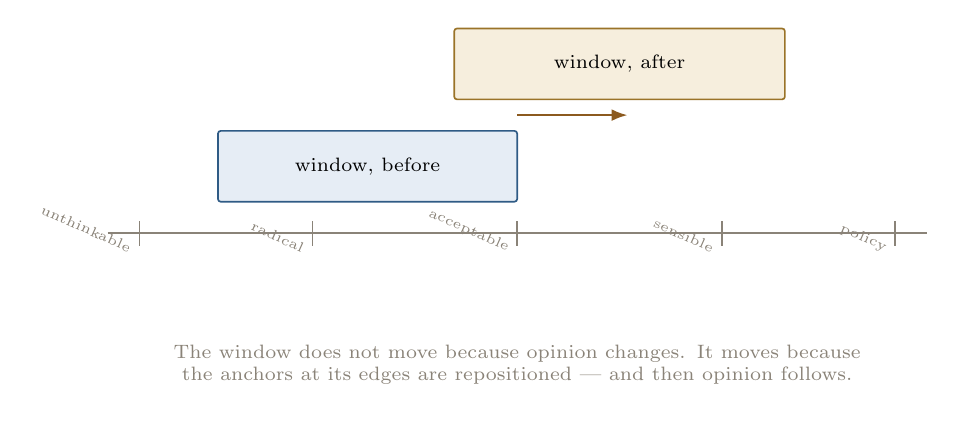
\begin{tikzpicture}[x=1mm, y=1mm, font=\sffamily\footnotesize]
  \draw[tksMuted, line width=0.6pt] (0,0) -- (104,0);
  \foreach \x/\lab in {4/unthinkable, 26/radical, 52/acceptable,
                       78/sensible, 100/policy} {
    \draw[tksMuted, line width=0.5pt] (\x,-1.6) -- (\x,1.6);
    \node[anchor=north, font=\tiny, text=tksMuted, rotate=-24, anchor=east]
      at (\x,-2.4) {\lab};
  }
  \draw[fill=tksBfill, draw=tksBedge, line width=0.6pt, rounded corners=1pt]
    (14,4) rectangle (52,13);
  \node[font=\scriptsize] at (33,8.5) {window, before};
  \draw[fill=tksAfill, draw=tksAedge, line width=0.6pt, rounded corners=1pt]
    (44,17) rectangle (86,26);
  \node[font=\scriptsize] at (65,21.5) {window, after};
  \draw[-{Latex[length=2mm]}, tksAccent, line width=0.7pt] (52,15) -- (66,15);
  \node[anchor=north, text width=94mm, align=center, font=\scriptsize,
        text=tksMuted] at (52,-13)
    {The window does not move because opinion changes. It moves because the
     anchors at its edges are repositioned --- and then opinion follows.};
\end{tikzpicture}
\end{document}
